\chapter{Preliminaries}
\label{Basics}

This chapter provides basic facts on Fourier analysis on the two-dimensional
sphere $\twosphere$ and related topics. Section \ref{Basics:Notation} 
familiarizes with elementary concepts and notational conventions. In Section \ref{Basics:LegendreTypeFunctions} we introduce \emph{Legendre functions} 
which in Section \ref{Basics:SphericalHarmonics} lead to the standard basis 
of \emph{spherical harmonics} on the sphere $\twosphere$, namely the
\emph{spherical surface functions}. The concept of \emph{spherical 
radial basis functions} is explained in Section \ref{Basics:SphericalKernels}
and accompanied by examples. 

We mention \emph{discrete cosine transforms} and a related algorithm
for fast multiplication of polynomials in Sections 
\ref{Basics:DiscreteCosineTransform} and 
\ref{Basics:FastPolynomialMultiplication},respectively, and close with a short glance at 
the fast Fourier transformation for nonuniform nodes (NFFT) in Section
\ref{Basics:NFFT}.

\section{Notational Conventions}
\label{Basics:Notation}

Every point $\V{x} \in \R^3 \setminus \set{\V{0}}$ given in \emph{Cartesian
coordinates} by the vector $\paren{x_1,x_2,x_3}^{\transp}$ can be described 
in emph{spherical coordinates} by a vector $\paren{r,\vtheta,\vphi}^{\transp}$ with 
the radius $r \in \Rp$ and the angles $\vtheta \in \interv{[}{0}{\pi}{]}$, $\vphi \in \interv{[}{0}{2\pi}{)}$.
We have
\begin{eqnarray*}
  \paren{x_1,x_2,x_3}^{\transp} & = & \paren{r \sin \vtheta \cos \vphi, r \sin \vtheta \sin \vphi, r \cos \vtheta}^{\transp}\\
  r & = & \sqrt{x_1^2+x_2^2+x_3^2} = \norm{\V{x}}_2.
\end{eqnarray*} 
We denote by $\twosphere$ the two-dimensional unit sphere embedded into $\R^3$, i.e. 
\[\twosphere := \pset{\V{x} \in \R^{3}}{|}{\norm{\V{x}}_2=1}\] 
and identify a point $\V{\xi} \in \twosphere$ with the corresponding vector $\paren{\vtheta,\vphi}^{\transp}$. The 
spherical coordinate system is illustrated in Figure \ref{sphere}.

Now let $\V{\xi} := \paren{\vtheta,\vphi}^{\transp}$, $\V{\eta} := \paren{\vtheta',\vphi'}^{\transp} \in
\twosphere$ and let $\alpha = \fun{\angle}{\V{\xi},\V{\eta}}$ be the angle spanned by the origin, $\V{\xi}$ and $\V{\eta}$.
Then the standard inner product
$\V{\xi} \cdot \V{\eta} = \cos \alpha$ is given by
\begin{equation}
  \nonumber
  \cos \alpha = \cos\vtheta\cos\vtheta' +
  \sin\vtheta\sin\vtheta'\fun{\cos}{\vphi-\vphi'}.
\end{equation}

The space of \emph{homogeneous polynomials} of degree $k \in \NZ$ in $\R^3$ is denoted by
$\fun{\text{Hom}_k}{\R^3}$, comprising all polynomials $p_k \in \Pol_{k}\paren{\R^3}$ fulfilling 
$\fun{p_k}{\alpha\:\V{x}} = \alpha^k \fun{p_k}{\V{x}}$ for arbitrary $\alpha \in \R$ and $\V{x}
\in \R^3$. The proper subspace of \emph{harmonic homogeneous polynomials} of
degree $k$ is defined by
\begin{equation}
  \nonumber
  \fun{\text{Harm}_k}{\R^3} := \pset{p_k \in \fun{\text{Hom}_k}{\R^3}}{|}{\Delta p_{k} = 0},
\end{equation}
where $\Delta$ is the Laplacian
\begin{equation}
  \nonumber
  \Delta = \frac{\partial^2}{\partial x_1^2} + \frac{\partial^2}{\partial x_2^2} +
  \frac{\partial^2}{\partial x_3^2}.
\end{equation}
Furthermore, we have
\begin{align}
  \nonumber
  \fun{\dim}{\fun{\text{Hom}_k}{\R^3}} = \frac{(k+1)(k+2)}{2},\quad
  \fun{\dim}{\fun{\text{Harm}_k}{\R^3}} = 2k+1.
\end{align}
To keep it short, we let $\Pol_{k}\paren{\twosphere} := \left.\Pol_{k}\paren{\R^3}\right|_{\twosphere}$ and 
$\mathcal{H}_k := \left.\fun{\text{Harm}_k}{\R^3}\right|_{\twosphere}$. For 
more information we refer the reader to \cite{co}. A comprehensive introduction to spherical approximation is found in \cite{frgesc}.

\begin{figure}[tb]
  \centering
  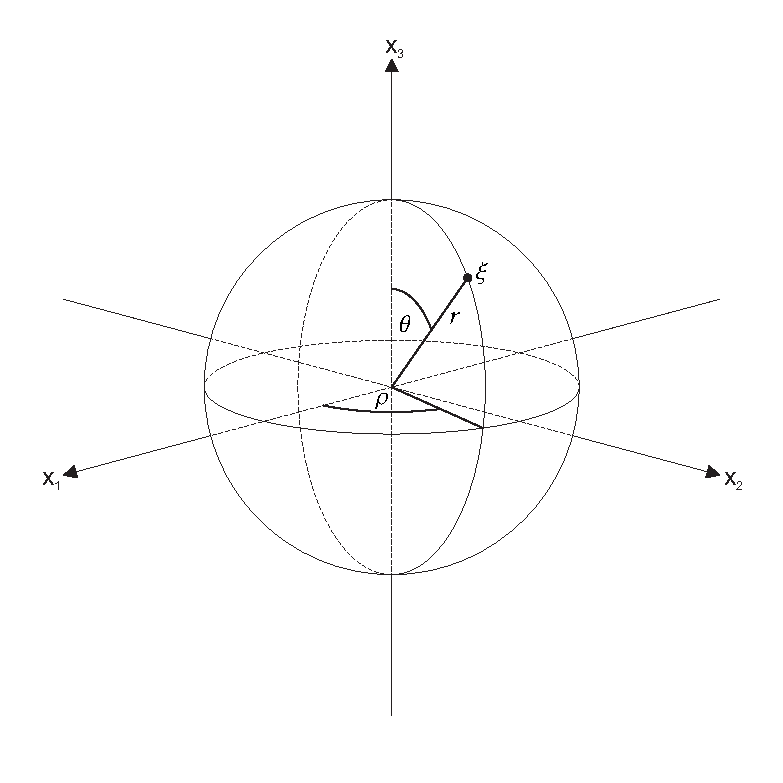
\includegraphics[width=0.87\textwidth]{images/sphere}
  \caption{The spherical coordinate system in $\R^3$: Every point $\V{\xi}$ on a
  sphere with radius $r$ centered at the origin can be described by angles 
  $\vtheta \in [0,\pi]$, $\vphi \in [-\pi,\pi)$ and the radius $r \in \Rp$. 
  For $\vtheta = 0$ or $\vtheta = \pi$ the point $\V{\xi}$ coincides with the 
  North or the South pole, respectively.}
  \label{sphere}
\end{figure}

Throughout this text, vectors $\V{x}$ and matrices $\V{A}$ are printed 
in boldface. Explicitly represented matrices with scalar entries are 
delimited by parenthesis $($ and $)$ whereas block matrices composed of matrices 
themselves are delimited by braces $[$ and $]$. Let now $j,k,m,n \in \N$. As usual, $\V{0}$ is the \emph{null vector}
$\paren{0,0,\ldots,0}^{\transp} \in \R^{n}$ and $\V{I}_{n}$ is the 
$n$-dimensional \emph{identity matrix} 
\[
  \V{I}_{n} := 
    \left(\begin{array}{cccc}
         1 &        0 &  \dots &       0\\
           0 &      1 & \ddots &  \vdots\\
      \vdots & \ddots & \ddots &       0\\
           0 &  \dots &      0 &       1\\
    \end{array}\right) \in \R^{n \times n}.
\]
The \emph{Kronecker product} $\V{A} \otimes \V{B}$ of two matrices 
$\V{A} := \paren{a_{ij}} \in \R^{j \times k}$ and 
$\V{B} \in \R^{m \times n}$ is defined by
\[
  \V{A}\otimes \V{B} := 
    \left[\begin{array}{ccc}
      a_{1,1} \V{B} & \dots & a_{1,k} \V{B} \\
             \vdots & \ddots & \vdots \\
      a_{j,1} \V{B} & \dots & a_{j,k} \V{B} \\
    \end{array}\right] \in \R^{(j+m)\times(k+n)}
\]
For a vector $\V{x} = \paren{x_{j}}_{j=0}^{n-1} 
\in \C^{n}$, we denote by $\V{W} = \fun{\diag}{\V{x}}$ or
$\V{W} = \fun{\diag}{x_{j}}$ 
the diagonal matrix
\[
  \V{W} := 
    \left(\begin{array}{cccc}
       x_{0} &      0 &  \dots &       0\\
           0 &  x_{1} & \ddots &  \vdots\\
      \vdots & \ddots & \ddots &       0\\
           0 &  \dots &      0 & x_{n-1}\\
    \end{array}\right) \in \C^{n \times n}.
\]
Moreover, $\norm{\cdot}_{1}$, $\norm{\cdot}_{2}$ and $\norm{\cdot}_{\infty}$
denote the usual \emph{$1$-norm}, \emph{Euclidean} or \emph{$2$-norm}, 
and the \emph{infinity-} or \emph{maximum-norm},
respectively. For a matrix $\V{W} = \fun{\diag}{w_{j}} \in
{\R}^{n}$ with $w_{j} > 0$ the \emph{weighted Euclidean norm}
 $\norm{\cdot}_{\V{W}}$ is understood as $\norm{\cdot}_{\V{W}} 
 := \norm{\V{W}^{1/2}\:\cdot\;}_{2}$.
 
The \emph{range} $\fun{\mathcal{R}}{A}$ and \emph{nullspace}
$\fun{\mathcal{N}}{A}$
of a matrix $\V{A} \in \C^{n \times n}$ is given by
\begin{align*} 
  \fun{\mathcal{R}}{A} & := \pset{\V{y} = \V{A}\:\V{x}}{|}{\V{x} \in \C^{n}},\\
  \fun{\mathcal{N}}{A} & := \pset{\V{x} \in \C^{n}}{|}{\V{A}\:\V{x} = \V{0}}.
\end{align*}
For the fundamental identity $\fun{\mathcal{R}}{A} = \fun{\mathcal{N}}{A^{\h}}$
we refer the reader to \cite{bjoerk}.

\section{Legendre Functions}
\label{Basics:LegendreTypeFunctions}
In this section, we briefly introduce \emph{Legendre polynomials}, \emph{associated Legendre functions} 
and \emph{associated Legendre polynomials} and collect basic properties. These functions play 
a major role in Fourier analysis on the sphere and are key for the algorithms related to spherical Fourier 
expansions, developed in this text.

The Legendre polynomials $P_k : \interv{[}{-1}{1}{]} \rightarrow \R$, $k \in \N_{0}$ 
as \emph{classical orthogonal polynomials} are given by their corresponding 
\emph{Rodrigues formula}
\begin{equation}
  \nonumber
  \fun{P_k}{x} := \frac{1}{2^k k!} \frac{\dx^k}{\dx x^k} \paren{x^2-1}^k.
\end{equation}
One verifies $\fun{P_{k}}{\pm1} = \paren{\pm1}^{k}$, $\left|\fun{P_{k}}{\cos\vartheta}\right|
\le \sqrt{\frac{2}{\pi k \sin\vartheta}}$ for $\vartheta \in (0,\pi)$ and $k \ge 1$, 
and $\max_{x \in \interv{[}{-1}{1}{]}} \abs{\fun{P_{k}}{x}} = 1$ (see \cite[pp. 47]{niuv}).
For convenience, we let $\fun{P_{-1}}{x} := 0$. Two recurrence relations are given by
\begin{equation}
  \label{three1}
  \paren{k+1}\fun{P_{k+1}}{x} = \paren{2k+1}x\fun{P_{k}}{x} - k\fun{P_{k-1}}{x} \quad \paren{k \in \NZ}
\end{equation}
and
\begin{equation}
  \label{three2}
  \paren{2k+1} \fun{P_{k}}{x} = \fun{P_{k+1}'}{x} - \fun{P_{k-1}'}{x}  \quad \paren{k \in \NZ}.
\end{equation}
Furthermore, we define the associated Legendre functions $P_k^n : \interv{[}{-1}{1}{]} \rightarrow \R$ by
\begin{equation}
  \label{basics:AssLegDef}
  \fun{P_k^n}{x} := \paren{\frac{\paren{k-n}!}{\paren{k+n}!}}^{1/2}
  \paren{1-x^2}^{n/2} \frac{\dx^n}{\dx x^n} \fun{P_k}{x} \quad \paren{n \in \NZ,\ k \ge n}.
\end{equation}
For fixed $n$, the set $\set{P_{k}^n}_{k \ge n}$ forms a complete set of orthogonal functions for $\Ln{2}{[-1,1]}$ with
\[ 
  \scalarproduct{P_{k}^n}{P_{l}^n}_{\Ln{2}{[-1,1]}} := \int_{-1}^{1} \fun{P_{k}^n}{x} 
  \fun{P_{l}^n}{x} \dx x = \frac{2}{2k+1} \delta_{k,l} \quad \paren{0 \le n \le k,l}.
\]
The associated Legendre functions obey the three-term recurrence relation
\begin{equation}
  \label{Basics:AssociatedLegendreDefinition}
    \fun{P_{k+1}^n}{x} = v_{k}^n x \fun{P_{k}^n}{x} + w_{k}^n 
    \fun{P_{k-1}^n}{x} \quad (k \ge n),
\end{equation}
with $\fun{P_{n-1}^n}{x} := 0$, $\fun{P_{n}^n}{x} = 
\frac{\sqrt{(2n)!}}{2^n n!} \paren{1-x^2}^{n/2}$, and
\begin{equation} 
  \label{Basics:AssociatedLegendreRecurrenceCoefficients}
v_{k}^n := \frac{2k+1}{((k-n+1)(k+n+1))^{1/2}}\; ,\qquad w_{k}^n := - \frac{((k-n)(k+n))^{1/2}}{((k-n+1)(k+n+1))^{1/2}}.
\end{equation}
A simple but at the same time powerful idea is to define the associated Legendre functions $P_k^n$ also for 
$k < n$ by means of the modified three-term recurrence relation
\begin{equation} 
  \label{Basics:AssociatedLegendreDefinitionExtended}
  \fun{P_{k+1}^n}{x} = \paren{\alpha_{k}^n x + \beta_{k}^n} \fun{P_{k}^n}{x} + \gamma_{k}^n \fun{P_{k-1}^n}{x}\quad\paren{k \in \NZ}
\end{equation}
with
\begin{equation}
  \label{Basics:AssociatedLegendreRecurrenceCoefficientsExtended}
  \begin{split}
	  \alpha_{k}^n & := \left\{
	    \begin{array}{ll}
	      (-1)^{k+1} & \text{for}\ k < n,\\
	      v_{k}^n    & \text{otherwise},
	    \end{array}\right.\\
	  \beta_{k}^n & := \left\{
	    \begin{array}{lll}
	      1 & \text{for}\ k < n,\\
	      0 & \text{otherwise},
	    \end{array}\right.\\
	  \gamma_{k}^n & := \left\{
	    \begin{array}{lll}
	      0       & \text{for}\ k \leq n,\\
	      w_{k}^n & \text{otherwise.}
	    \end{array}\right.
	\end{split}  
\end{equation}
For even $n$, we let
\[ 
  \fun{P_{-1}^n}{x} := 0,\ \fun{P_{0}^n}{x} := \frac{\sqrt{(2n)!}}{2^n n!},
\]
and for odd $n$, we start with
\[ \fun{P_{0}^n}{x} := \fun{P_{1}^n}{x} := \frac{\sqrt{(2n)!}}{2^n n!} \paren{1-x^2}^{1/2},\]
where $\fun{P_{-1}^n}{x} := 0$ is understood.
For $k \ge n$, this definition coincides with \eqref{Basics:AssociatedLegendreDefinition}. 
As a matter of fact, $P_{k}^n$ is a polynomial of degree $k$, if $n$ is even, while 
$\paren{1-x^2}^{-1/2}P_{k}^n$ is a polynomial of degree $k-1$ for odd $n$, as
easily verified by \eqref{basics:AssLegDef}.

Based on the recurrence coefficients from \eqref{Basics:AssociatedLegendreRecurrenceCoefficientsExtended} 
and introducing a shift parameter $c \in \NZ$, we 
define the associated Legendre polynomials $\fun{P_{k}^n}{\cdot,c}$ by
\begin{equation}
  \label{Basics:AssociatedLegendrePolynomials}
  \begin{split}
    & \fun{P_{-1}^n}{x,c} := 0,\ \fun{P_{0}^n}{x,c} := 1,\\
    & \fun{P_{k+1}^n}{x,c} = \paren{\alpha_{k+c}^n x + \beta_{k+c}^n} \fun{P_{k}^n}{x,c} + \gamma_{k+c}^n \fun{P_{k-1}^n}{x,c} \quad \paren{k \in \N}.
  \end{split}
\end{equation}
\newpage
We have the following Lemma:
\begin{lemma}
  \label{Basics:AssociatedLegendreRecurrence}
  Let $c,k,n \ge 0$ and let the functions $P_{k}^n$ and 
  $\fun{P_{k}^n}{\cdot,c}$ be given as in 
  \eqref{Basics:AssociatedLegendreDefinitionExtended}, 
  \eqref{Basics:AssociatedLegendreRecurrenceCoefficientsExtended}, and 
  \eqref{Basics:AssociatedLegendrePolynomials}. 
  Then we have
  \[ 
    \fun{P_{c+k}^n}{x} = \fun{P_{k}^n}{x,c} \fun{P_{c}^n}{x} + \gamma_{c}^n \fun{P_{k-1}^n}{x,c+1} \fun{P_{c-1}^n}{x}.
  \]
\end{lemma}
\begin{proof}
  The proof is by induction over $k$. So let $c \ge 0$ be arbitrary. 
  For $k = 0,1$ we have
  \begin{align*}
    \nonumber
    \fun{P_{c+0}^n}{x} 
    & = 1 \cdot \fun{P_{c}^n}{x} + \gamma_{c}^n \cdot 0 \cdot \fun{P_{c-1}^n}{x}\\
    & = \fun{P_{0}}{x,c}\fun{P_{c}^n}{x} + \gamma_{c}^n \fun{P_{-1}}{x,c} \fun{P_{c-1}^n}{x},\\
    \fun{P_{c+1}^n}{x} 
    & = \paren{\alpha_{c}^n x + \beta_{c}^n} \fun{P_{c}^n}{x} + \gamma_{c}^n \fun{P_{c-1}^n}{x}\\
    \nonumber
    & = \fun{P_{1}}{x,c}\fun{P_{c}^n}{x} + \gamma_{c}^n \fun{P_{0}}{x,c} \fun{P_{c-1}^n}{x}.
  \end{align*}
  Let now the assertion be true for $k$ and $k-1$, where $k \ge 1$ is fixed. We find
  \begin{equation}
    \nonumber
    \begin{split}
      \fun{P_{c+k+1}^n}{x}& 
       = \paren{\alpha_{c+k}^n x + \beta_{c+k}^n} \fun{P_{c+k}^n}{x} + \gamma_{c+k}^n \fun{P_{c+k-1}^n}{x}\\
      & = \paren{\alpha_{c+k}^n x + \beta_{c+k}^n} \paren{\fun{P_{k}^n}{x,c} \fun{P_{c}^n}{x} + 
      \gamma_{c}^n \fun{P_{k-1}^n}{x,c+1} \fun{P_{c-1}^n}{x}}\\
      & \quad + \gamma_{c+k}^n \paren{\fun{P_{k-1}^n}{x,c} \fun{P_{c}^n}{x} + 
      \gamma_{c}^n \fun{P_{k-2}^n}{x,c+1} \fun{P_{c-1}^n}{x}}\\
      & = \left[\paren{\alpha_{c+k}^n x + \beta_{c+k}^n}\fun{P_{k}^n}{x,c} + \gamma_{c+k}^n\fun{P_{k-1}^n}{x,c}\right]
       \fun{P_{c}^n}{x}\\ 
      & \quad + \gamma_{c}^n\left[\paren{\alpha_{c+k}^n x + \beta_{c+k}^n}\fun{P_{k-1}^n}{x,c+1} + 
      \gamma_{c+k}^n\fun{P_{k-2}^n}{x,c+1}\right]\fun{P_{c-1}^n}{x}\\ 
      & = \fun{P_{k+1}^n}{x,c} \fun{P_{c}^n}{x} + \gamma_{c}^n \fun{P_{k}^n}{x,c+1} \fun{P_{c-1}^n}{x}.
    \end{split}  
  \end{equation}
\end{proof}

\section{Spherical Harmonics}
\label{Basics:SphericalHarmonics}

\emph{Spherical harmonics} on the sphere $\twosphere$ arise the same way as complex exponentials 
$\e^{\im n x}$, $n \in \Z$, on the unit circle $\mathbb{S}^1$. In cartesian coordinates they are 
homogeneous harmonic polynomials in $\R^3$, but restricted to the sphere $\twosphere$. For a brief 
comprehensive introduction we refer to \cite{Mo99}. A more general and abstract treatment is
found in \cite{frgesc}.

In $\R^2$ a homogeneous harmonic polynomial $p_{n}$ of degree $n \in \NZ$ must fulfill 
\[
  \fun{p_{n}}{r,\vphi} = r^n \fun{q_{n}}{\vphi},\quad n^2 \fun{q_{n}}{\vphi} + \fun{q_{n}''}{\vphi} = 0
\]
in polar coordinates $r \in \Rp$, $\vphi \in [-\pi,\pi)$. Restricted to the unit circle $\mathbb{S}^1$, 
i.e. for $r=1$, $p_{n} = q_{n}$ is equivalently
an eigenfunction of the \emph{circular Laplacian} $\Delta_{\vphi} := \frac{\partial^2}{\partial \vphi^2}$ 
corresponding to the eigenvalue $n^2$.
Following these lines, a homogeneous harmonic polynomial $p_{k} \in \fun{\Pi}{\R^3}$ in spherical coordinates, 
restricted to the unit sphere $\twosphere$,
is an eigenfunction of the \emph{spherical Laplacian} or \emph{Laplace-Beltrami operator} 
\[
  \Delta_{\paren{\vtheta,\vphi}} := \frac{1}{\sin^2 \vtheta} 
  \frac{\partial^2}{\partial \vphi^2} + \frac{1}{ \sin \vtheta}�
   \frac{\partial}{\partial \vtheta} \paren{\sin \vtheta \: \frac{\partial}{\partial \vtheta}}.
\]
for the eigenvalue $k(k+1)$ and obeys
$\Delta_{\paren{\vtheta,\vphi}} p_{k} = -k(k+1) p_{k}$.
Using an ansatz based on separation of variables for the obtained partial differential equation
$\Delta_{\paren{\vtheta,\vphi}} p_{k} + k(k+1) p_{k} = 0$ (see \cite{co2}), one finds 
the linearly independent solutions
\begin{equation}
  \label{Basics:SphericalHarmonicsDefinition}
  \begin{split}
    & Y_{k}^n: \twosphere \rightarrow \C \quad \paren{k \in \NZ,\; n = -k,\ldots,k},\\
    & \fun{Y_{k}^n}{\vtheta,\vphi} := \sqrt{\frac{2k+1}{4\pi}} 
    \fun{P_{k}^{\abs{n}}}{\cos \vtheta} \e^{\im n \vphi},
  \end{split}
\end{equation}
called \emph{spherical surface functions}.
The index $k$ is called the \emph{degree} and $n$ is denoted the \emph{order} of $Y_{k}^n$. 
Figure \ref{Basics:Figure:SphericalHarmonics} illustrates some functions $Y_{k}^{n}$.
Due to the separability with respect to $\vtheta$ and $\vphi$, one proves easily the 
orthogonality property
\begin{equation}
  \label{Basics:orthogonality}
  \scalarproduct{Y_{k}^n}{Y_{l}^m}_{\Ln{2}{\twosphere}} = \delta_{k,l} \delta_{n,m}
\end{equation}
with respect to the usual $\Ln{2}{\twosphere}$-inner product 
\begin{equation}
  \nonumber
  \scalarproduct{Y_{k}^n}{Y_{l}^m}_{\Ln{2}{\twosphere}} = \int_{\twosphere}
  \fun{Y_{k}^n}{\V{\xi}} \overline{\fun{Y_{l}^m}{\V{\xi}}} \: \dx \V{\xi} := 
  \int_{0}^{2\pi} \int_{0}^{\pi} \fun{Y_{k}^n}{\vtheta,\vphi} 
  \overline{\fun{Y_{l}^m}{\vtheta,\vphi}} \sin \vtheta \; 
  \dx \vtheta \; \dx \vphi.
\end{equation}
Recall that for $k \in \NZ$ we denote by $\mathcal{H}_{k}$ the space of harmonic homogeneous 
polynomials of degree $k$ restricted to the sphere $\twosphere$. An important result states 
that $Y_{k}^n \in \mathcal{H}_k$ for $n = -k,\ldots,k$, and therefore, the set
\begin{equation}
  \nonumber
  \pset{Y_{k}^n}{|}{n = -k,\ldots,k}
\end{equation}
constitutes an orthonormal basis of $\mathcal{H}_k$, owing to $\dim \mathcal{H}_k =
2k+1$. Moreover, due to \eqref{Basics:orthogonality}, the spaces $\mathcal{H}_k$ are orthogonal
to each other and
\begin{equation}
  \label{Basics:FourierBasis}
  \pset{Y_{k}^n}{|}{k = 0,\ldots,M;\ n = -k,\ldots,k} \quad \paren{M \in \NZ}
\end{equation}
provides an orthonormal basis for the space $\bigoplus_{k=0}^{M}\mathcal{H}_k$, called
the space of \emph{spherical harmonics} of degree $M$.

At first glance, the restriction to homogeneous and harmonic polynomials
might exclude various functions from $\fun{\Pol_M}{\twosphere}$. But as a 
matter of fact, these spaces are identical (see \cite[Corollary 2.2.5]{frgesc}), i.e. 
\begin{equation}
  \nonumber
    \fun{\Pol_M}{\twosphere} = \bigoplus_{k=0}^{M}\mathcal{H}_k \quad \paren{M \in \NZ}.
\end{equation}
Since polynomials are dense in $\Ln{2}{\twosphere}$, we have also obtained an orthonormal 
basis for $\Ln{2}{\twosphere}$ and we call 
\[
  \pset{Y_{k}^n}{|}{k \in \NZ,\ n = -k,\ldots,k}
\]
the \emph{standard basis of spherical harmonics} or \emph{Fourier basis} 
for $\Ln{2}{\twosphere}$. Therefore, a function $f \in \Ln{2}{\twosphere}$ can be 
developed into a series
\[
  f = \sum_{k=0}^{\infty} \sum_{n=-k}^{k} a_{k}^n Y_{k}^n,
\]
where the coefficients $a_{k}^n := \fun{f^{\wedge}}{k,n} := \scalarproduct{f}{Y_{k}^{n}}_{\Ln{2}{\twosphere}}$
are the \emph{spherical Fourier coefficients} and the equivalence is understood in the $\text{\rm{L}}^2$-sense.

\begin{figure}[hp]
  \centering
   \subfigure[$\Re \: Y_{0}^{0}$]
     {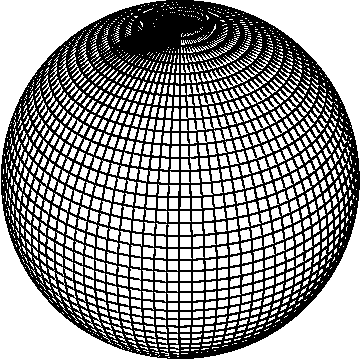
\includegraphics[width=0.33\textwidth]{images/sh_r_0_0}}\hfill
   \subfigure[$\Re \: Y_{4}^{2}$]
     {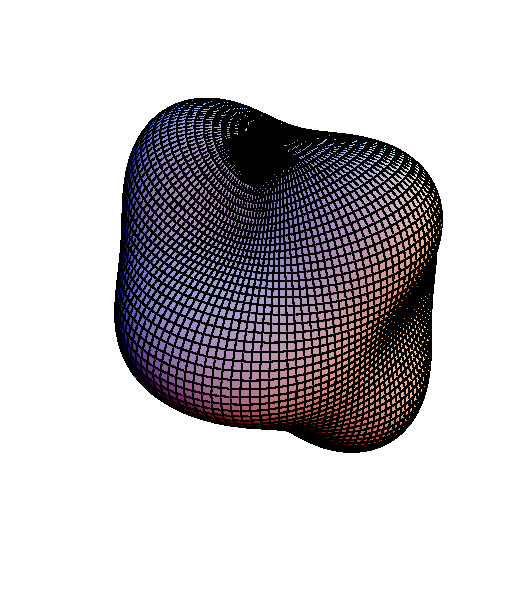
\includegraphics[width=0.33\textwidth]{images/sh_r_4_2}}\\
   \subfigure[$\Re \: Y_{9}^{5}$]
     {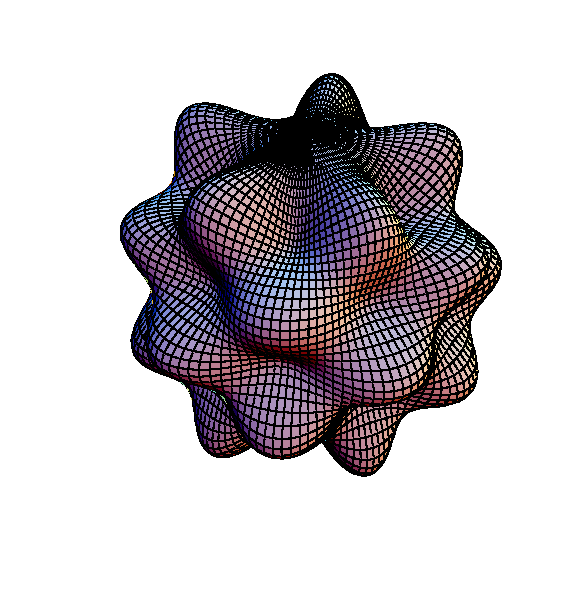
\includegraphics[width=0.33\textwidth]{images/sh_r_9_5}}\hfill
   \subfigure[$\Re \: Y_{13}^{1}$]
     {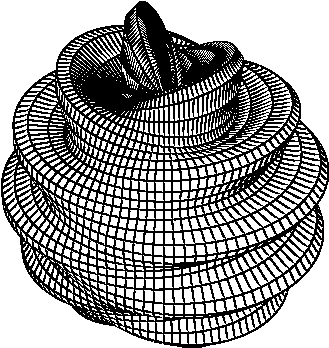
\includegraphics[width=0.33\textwidth]{images/sh_r_13_1}}\\
   \subfigure[$\Re \: Y_{13}^{6}$]
     {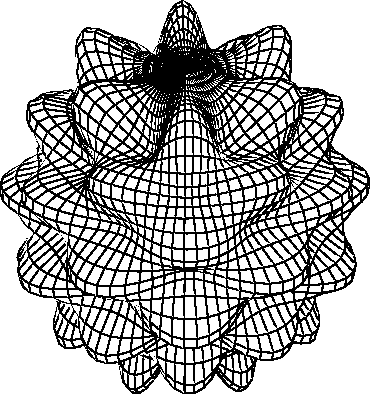
\includegraphics[width=0.33\textwidth]{images/sh_r_13_6}}\hfill
   \subfigure[$\Re \: Y_{13}^{13}$]
     {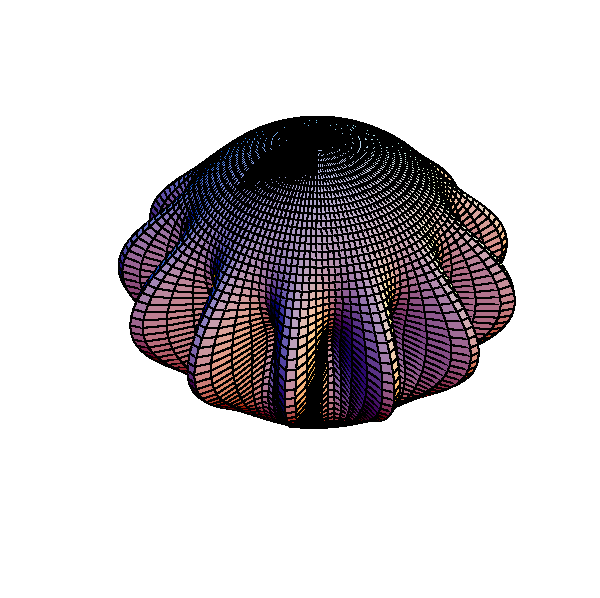
\includegraphics[width=0.33\textwidth]{images/sh_r_13_13}}\\
  \caption{The real part of $Y_{k}^{n}$ for different combinations $\paren{k,n}$.}
  \label{Basics:Figure:SphericalHarmonics}
\end{figure}

We finally mention the fundamental and well known \emph{Addition Theorem} for spherical harmonics 
that relates any set of functions $\set{H_k^n}_{n=-k}^k$ forming an orthonormal basis of the space $\mathcal{H}_k$ 
to the Legendre polynomial $P_{k}$.

\begin{proposition}[Addition Theorem]
  \label{Basics:AdditionTheorem}
  Let $k \in \NZ$ and $\V{\xi}, \V{\eta} \in \twosphere$. For every 
  $\Ln{2}{\twosphere}$-orthonormal basis $\set{H_{k}^n}_{n=-k}^{k}$ of 
  $\mathcal{H}_k$, we have
  \begin{equation}
    \nonumber
    \sum_{n=-k}^{k} \fun{H_{k}^n}{\V{\xi}} \overline{\fun{H_{k}^n}{\V{\eta}}} =
    \frac{2k+1}{4\pi}\fun{P_k}{\V{\xi} \cdot \V{\eta}}.
  \end{equation}
\end{proposition}

See \cite[p. 37]{frgesc} or \cite[pp. 172, Theorem 5]{co} for a proof. In particular, the theorem 
holds for the spherical surface functions $Y_{k}^n$.

\section{Spherical Radial Basis Functions}
\label{Basics:SphericalKernels}

\emph{Spherical radial basis functions} are the spherical counterpart 
of \emph{radial basis functions} in Euclidean spaces (see for example 
\cite{buhmann} or \cite{wendland}). Other synonymous denotations are \emph{spherical radial kernels} or
\emph{zonal functions}.
Generally, one starts with a function $K$ from $\Ln{2}{\interv{[}{-1}{1}{]}}$
and defines for a fixed point $\V{\eta} \in \twosphere$ the \emph{$\V{\eta}$-zonal} function 
\[
  \fun{K}{\V{\eta} \: \cdot}: \twosphere \rightarrow \C,\ \V{\xi} \mapsto \fun{K}{\V{\eta} \cdot \V{\xi}} \quad \paren{\V{\xi} \in \twosphere}.
\]
The fact that the geodesic distance $\fun{d}{\V{\eta},\V{\xi}}$ for two points $\V{\eta}$, $\V{\xi} \in \twosphere$ is $\fun{d}{\V{\eta},\V{\xi}} = 
\sqrt{2-2\V{\eta}\cdot\V{\xi}}$ justifies the name \emph{spherical radial basis function}. 
By means of the \emph{Funk-Hecke formula} (see \cite[pp. 60]{frgesc}) we obtain for fixed $k \in \NZ$
\begin{equation}
  \label{Basics:Symbol2}
  \scalarproduct{\fun{K}{\V{\eta} \: \cdot}}{Y_{k}^n}_{\Ln{2}{\twosphere}} = \int_{\twosphere} 
  \fun{K}{\V{\eta} \cdot \V{\xi}} \overline{\fun{Y_{k}^n}{\V{\xi}}} \: \dx \V{\xi} = 
  \fun{K^{\wedge}}{k} \overline{\fun{Y_{k}^n}{\V{\eta}}} \quad \paren{n=-k,\ldots,k},
\end{equation}
where the \emph{Legendre transform} $K^{\wedge}$ of $K$ is given by
\begin{equation}
  \label{Basics:Symbol}
  \fun{K^{\wedge}}{k} := 2 \pi \int_{-1}^{1} \fun{K}{x} \fun{P_{k}}{x} \dx x \quad \paren{k \in \NZ}.
\end{equation}
We have therefore the representation
\begin{equation}
  \label{Basics:Kernel}
  \fun{K}{\V{\eta} \cdot \V{\xi}} = \sum_{k = 0}^{\infty} \sum_{n=-k}^k \fun{K^{\wedge}}{k} 
  \overline{\fun{Y_{k}^n}{\V{\eta}}} \fun{Y_{k}^n}{\V{\xi}} 
\end{equation}
and by applying the Addition Theorem from Proposition \ref{Basics:AdditionTheorem} we obtain 
for $K$ the orthogonal expansion
\begin{equation}
\label{Basics:OrthogonalKernelExpansion}
  \fun{K}{\V{\eta} \cdot \V{\xi}} = \sum_{k = 0}^{\infty} \frac{2k+1}{4\pi} \fun{K^{\wedge}}{k} \fun{P_k}{\V{\eta} \cdot \V{\xi}}.
\end{equation}
\begin{remark}
  In other contexts, the name \emph{Legendre transform} often refers to a different type of function transformation.
  In our setting, the Legendre transform $\fun{K^{\wedge}}{k}$ is also called the $symbol$ of $K$ since it corresponds to a
  linear operator $\Lambda: \Ln{2}{\twosphere} \rightarrow \Ln{2}{\twosphere}$ with 
  $\fun{\paren{\Lambda f}^{\wedge}}{k,n} = \fun{K^{\wedge}}{k} \fun{f^{\wedge}}{k,n}$.
\end{remark}
The symbol $\fun{K^{\wedge}}{k}$ has many remarkable properties. The following result allows for the 
construction of so-called \emph{iterated spherical radial basis functions} by multiplying the corresponding symbols (see \cite{frsc}).
\begin{lemma}
  Let $P,Q\in \Ln{2}{\interv{[}{-1}{1}{]}}$ and
  \[
  \fun{K}{\V{\eta} \cdot \V{\xi}} := \fun{\left(P * Q\right)}{\V{\eta} \cdot
    \V{\xi}},
  \]
  where
  \begin{equation}
    \label{Basics:Convolution}
    \fun{\left(P * Q\right)}{\V{\eta} \cdot \V{\xi}}:= 
    \int_{\twosphere} \fun{P}{\V{\eta} \cdot \V{\nu}}
    \fun{Q}{\V{\nu} \cdot \V{\xi}} \dx \V{\nu}
  \end{equation}
  is the \emph{spherical convolution} of $Q$ and $P$. Then the symbol 
  $\fun{K^{\wedge}}{k}$ is given by 
  $\fun{K^{\wedge}}{k} = \fun{P^{\wedge}}{k} \fun{Q^{\wedge}}{k}$.
  Furthermore, for compactly supported functions with $\supp\; P = \supp\; Q =
  \interv{[}{h}{1}{]}$, $h \in [0,1]$, we have $\supp\; K =
  \interv{[}{2h^2-1}{1}{]}$.
\end{lemma}
\begin{proof}
  First, we use \eqref{Basics:Symbol2} and obtain
  \begin{equation}
    \begin{split}
      \scalarproduct{\fun{K}{\V{\eta} \: \cdot}}{Y_{k}^n}_{\Ln{2}{\twosphere}} 
      & = \int_{\twosphere} \fun{K}{\V{\eta} \cdot \V{\xi}} \overline{\fun{Y_{k}^n}{\V{\xi}}} \: \dx \V{\xi}\\
      & = \int_{\twosphere} \int_{\twosphere} \fun{P}{\V{\eta} \cdot \V{\nu}}
          \fun{Q}{\V{\nu} \cdot \V{\xi}} \: \dx \V{\nu} \; \overline{\fun{Y_{k}^n}{\V{\xi}}} \: \dx \V{\xi}\\
      & = \int_{\twosphere} \int_{\twosphere} \fun{Q}{\V{\nu} \cdot \V{\xi}} \overline{\fun{Y_{k}^n}{\V{\xi}}} \:
          \dx \V{\xi} \; \fun{P}{\V{\eta} \cdot \V{\nu}} \: \dx \V{\nu}\\
      & = \int_{\twosphere} \fun{Q^{\wedge}}{k} \fun{P}{\V{\eta} \cdot \V{\nu}} 
          \overline{\fun{Y_{k}^n}{\V{\nu}}} \: \dx \V{\nu}\\
      & = \fun{Q^{\wedge}}{k} \fun{P^{\wedge}}{k} \overline{\fun{Y_{k}^n}{\V{\eta}}}, 
    \end{split}
  \end{equation}  
  which proves $\fun{K^{\wedge}}{k} = \fun{P^{\wedge}}{k} \fun{Q^{\wedge}}{k}$. 
  If $P$ and $Q$ are compactly supported with $\supp\; P = \supp\; Q =
  \interv{[}{h}{1}{]}$, and $h \in [0,1]$, we note that the support of $P$ and $Q$ 
  are the corresponding spherical caps $\fun{C_{\V{\eta}}}{h}$ and $\fun{C_{\V{\nu}}}{h}$, where
   $\fun{C_{\V{\eta}}}{h} := \pset{\V{\xi} \in \twosphere}{|}{\V{\eta} \cdot \V{\xi} \ge h}$. For the 
   integrand in \eqref{Basics:Convolution} not to vanish we must require $\V{\nu}$ and $\V{\xi}$ to lie in the 
   spherical caps $\fun{C_{\V{\eta}}}{h}$ and $\fun{C_{\V{\nu}}}{h}$, respectively. Equivalently, if we denote
   by $\alpha$, $\beta$, $\gamma$ the angles $\fun{\angle}{\V{\eta},\V{\nu}}$, $\fun{\angle}{\V{\nu},\V{\xi}}$, and
   $\fun{\angle}{\V{\eta},\V{\xi}}$, we conclude $\gamma \le \alpha + \beta \le 2 \arccos h$, where we note that
   this estimate is sharp. Since $\fun{\cos}{2 \arccos h} = 2h^2-1$, the support of $K$ is $\supp\; K = \interv{[}{2h^2-1}{1}{]}$.
\end{proof}

In the following we shall give some examples of spherical radial basis functions. All examples are taken from 
\cite{frgesc} or \cite{frsc}, respectively. 

We consider the generating series
\begin{equation}
  \label{Basics:GeneratingFunction}
  \fun{\phi}{h} := \sum_{k = 0}^{\infty} h^k \fun{P_k}{x} \quad \paren{x \in \interv{[}{-1}{1}{]}}
\end{equation}
which is absolutely and uniformly convergent for $h \in
\interv{(}{-1}{1}{)}$ with
\begin{equation}
  \label{Basics:Solution}
  \sum_{k = 0}^{\infty} h^k \fun{P_k}{x} = \frac{1}{\sqrt{1-2hx+h^2}}.
\end{equation}
This follows from the ordinary differential equation
\begin{equation}
\label{Basics:DifferentialEquation}
  \paren{1+h^2-2hx}\fun{\phi'}{h} = \paren{x-h}\fun{\phi}{h}
\end{equation}
obtained by differentiation with respect to $h$ and comparing coefficients in line with \eqref{Basics:GeneratingFunction}. Using the initial 
condition $\fun{\phi}{0}=1$ yields the unique solution \eqref{Basics:Solution} of \eqref{Basics:DifferentialEquation}.
The identity
\begin{equation}
  \label{Basics:PoissonIdentity}
  \sum_{k=0}^{\infty} \paren{2k+1} h^k \fun{P_k}{x} =
  \frac{1-h^2}{\paren{1-2hx+h^2}^{3/2}}
\end{equation}
follows easily. 
\begin{definition}
  Let $h \in \interv{(}{0}{1}{)}$. The function
  $Q_{h}:\interv{[}{-1}{1}{]} \rightarrow \R$ with
  \begin{equation}
    \label{PoissonKernel}
    \fun{Q_{h}}{x} := \frac{1}{4\pi} \frac{1-h^2}{\paren{1-2hx+h^2}^{3/2}} \quad 
    \paren{x \in \interv{[}{-1}{1}{]}}
  \end{equation}
  is called \emph{Poisson kernel}. 
\end{definition}
The symbol $\fun{Q_{h}^{\wedge}}{k}$ is given by $\fun{Q_{h}^{\wedge}}{k} = h^k$ as easily seen in 
\eqref{Basics:PoissonIdentity}.
We refer to Figure \ref{Basics:Figure:PoissonKernel}. The parameter $h$
allows for controlling the concentration of the function's energy around
$x = 1$. The Poisson kernel is a positive function and normalized with
\[
  \int_{\twosphere} \fun{Q_{h}}{\V{\eta} \cdot \V{\xi}} \dx \V{\xi} = 1 \quad \paren{\V{\eta} \in \twosphere}.
\]
Further properties with respect to localization and smoothness are derived in \cite[pp. 112]{frgesc}.
\begin{figure}[tb]
  \centering
  \subfigure[$h=0.5,0.7,0.8$.]
  {
  \label{Basics:Figure:PoissonKernel}
  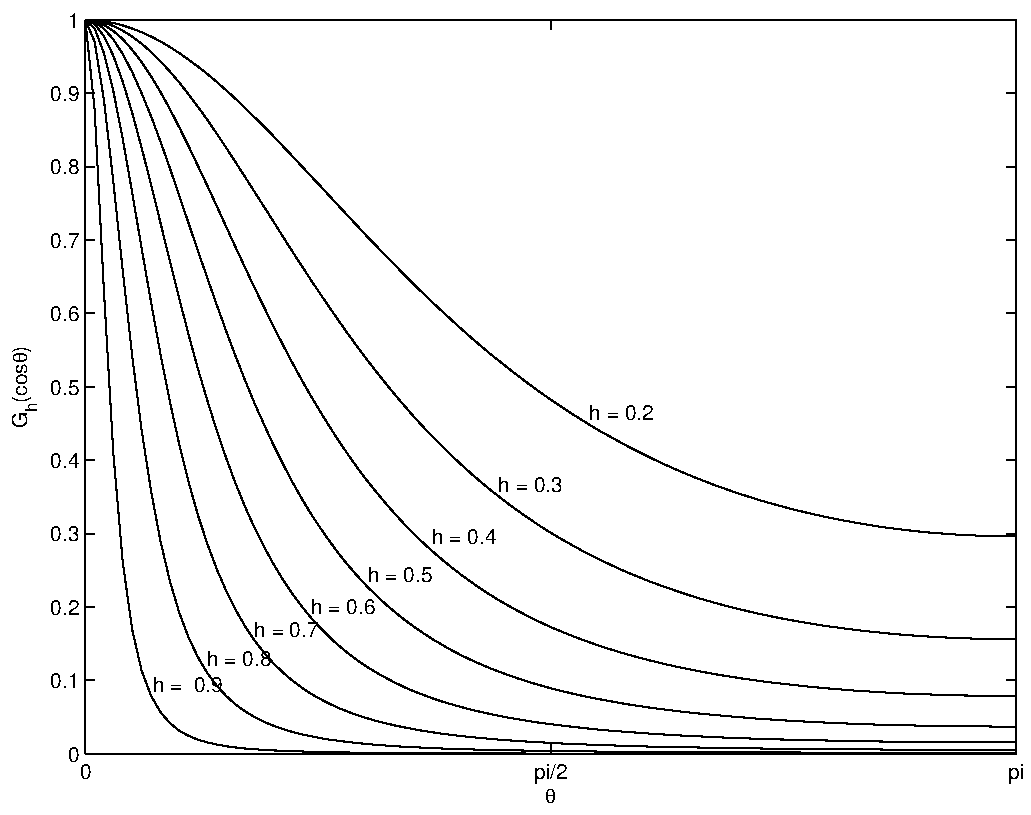
\includegraphics[width=0.45\textwidth]{images/poisson}
  }
  \hfill
  \subfigure[$h=0.8,0.9,0.955$.]
  {
    \label{Basics:Figure:SingularityKernel}
    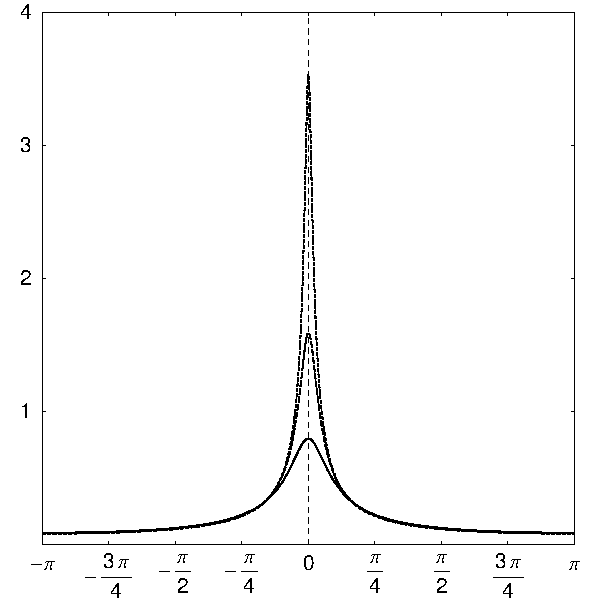
\includegraphics[width=0.45\textwidth]{images/singularity}
  }
  \caption{The kernels $\fun{Q_{h}}{\cos\vartheta}$ (left) and $\fun{S_{h}}{\cos\vartheta}$ (right)
  for different values of $h$.}
  \label{Basics:Figure:PoissonSingularityKernel}
\end{figure}
  The series \eqref{Basics:Solution} itself leads to a spherical radial basis function.
  \begin{definition}
    Let $h \in \interv{(}{0}{1}{)}$. The \emph{singularity kernel} 
    $S_{h}:\interv{[}{-1}{1}{]} \rightarrow \R$ is given by
    \begin{equation}
      \label{SingularityKernel}
      \fun{S_{h}}{x} := \frac{1}{2\pi} \sum_{k = 0}^{\infty} h^k \fun{P_k}{x} = 
      \frac{1}{2\pi} \frac{1}{\sqrt{1-2hx+h^2}} \quad \paren{x \in \interv{[}{-1}{1}{]}}.
    \end{equation}
  \end{definition}
  For the symbol $\fun{S_{h}^{\wedge}}{k}$, we have
  \[
    \fun{S_{h}^{\wedge}}{k} = \frac{2}{2k+1} h^k.
  \]
  See Figure \ref{Basics:Figure:SingularityKernel} and for more information \cite[pp. 112]{frgesc}.

  Locally supported zonal functions are considered for example in \cite{frsc}.
  \begin{definition}
    Let $h \in \interv{(}{0}{1}{)}$, $\lambda \in \Rp$, and $\mu \in \N$.
    \begin{enumerate}
	    \item Let the \emph{locally supported kernel}
	    $L_{h,\lambda}:\interv{[}{-1}{1}{]} \rightarrow \R$ be defined by
	    \[
	    \fun{L_{h,\lambda}}{x} := 
	    \left\{\begin{array}{l@{\quad \text{if} \quad}l} 
	        0 & -1 \le x \le h, \\
	        \frac{\lambda+1}{2\pi(1-h)^{\lambda+1}}\paren{x-h}^{\lambda} &  h <  x \le 1.
	      \end{array}\right.
	    \]
	    \item Furthermore, define the \emph{iterated locally supported kernels} 
	    $L_{h,\lambda}^{(\mu)}:\interv{[}{-1}{1}{]} \rightarrow \R$ recursively,
	    \[
	      L_{h,\lambda}^{(\mu+1)} := L_{h,\lambda}^{(\mu)} * L_{h,\lambda},
	    \]
	    where $L_{h,\lambda}^{(1)} := L_{h,\lambda}$.
    \end{enumerate}
  \end{definition}  
  
	Figures \ref{Basics:Figure:LKernel} and \ref{Basics:Figure:LKernelIterated} 
	show the 
	functions $L_{h,\lambda}$ for	different values $h$ and $\lambda$ and the 
	iterated kernel $L_{0.6,2}^{(\mu)}$ for different values of $\mu$, 
	respectively.
	While the parameter $h$ again steers the localization in spatial domain, the
	parameter $\lambda$ correponds to smoothness.
	The iterated kernel $L_{h,\lambda}^{(\mu)}$ trades localization in spatial domain
	for 'localization' in 'frequency domain', i.e. with respect to the symbol 
	$L_{h,\lambda}^{(\mu),\wedge}$.
	We mention the following lemma from \cite{frsc}:

	\begin{lemma}
	  The symbol $\fun{L_{h,\lambda}^{\wedge}}{k}$ can be computed recursively by
	    \[
	    \fun{L_{h,\lambda}^{\wedge}}{k+1} = \frac{\paren{2k+1} h}{k+\lambda+2}
	    \fun{L_{h,\lambda}^{\wedge}}{k}   - \frac{k-\lambda-1}{k+\lambda+2}
	    \fun{L_{h,\lambda}^{\wedge}}{k-1} \quad \paren{k \in \N},
	    \]
	    where $\fun{L_{h,\lambda}^{\wedge}}{0} = 1$ and
	    $\fun{L_{h,\lambda}^{\wedge}}{1} = \frac{\lambda + 1 + h}{\lambda+2}$.
	\end{lemma}
	
	\begin{proof}
	  We follow the lines in \cite{frsc}. Straightforward integration yields 
	  $\fun{L_{h,\lambda}^{\wedge}}{0} = 1$
	  and $\fun{L_{h,\lambda}^{\wedge}}{1} = \frac{\lambda + 1 + h}{\lambda+2}$.
	  We use \eqref{Basics:Symbol}, apply the recurrence relation \eqref{three1},
	  and find
	  \[
	    (k+1)\fun{L_{h,\lambda}^{\wedge}}{k+1} = (2k+1)\fun{L_{h,\lambda+1}^{\wedge}}{k} +
	    (2k+1)h\fun{L_{h,\lambda}^{\wedge}}{k} -k \fun{L_{h,\lambda}^{\wedge}}{k-1}.
	  \]
	  Next, using the recurrence relation \eqref{three2} and partial integration, we arrive at
	  \[
	    (2k+1)\fun{L_{h,\lambda+1}^{\wedge}}{k} = (\lambda+1)\paren{\fun{L_{h,\lambda}^{\wedge}}{k-1}-\fun{L_{h,\lambda}^{\wedge}}{k+1}}.
	  \]
	  The combination of these two results yields the assertion.
	\end{proof}

\begin{figure}[tb]
  \centering
   \subfigure[$\lambda=1$]
     {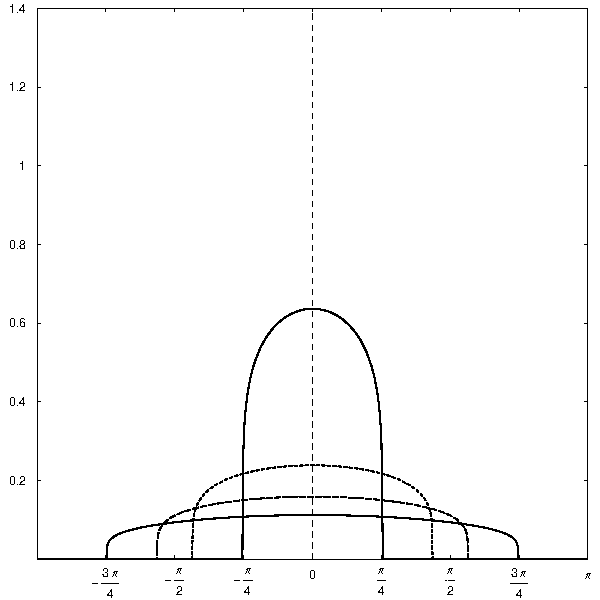
\includegraphics[width=0.45\textwidth]{images/locsup1}}\hfill
   \subfigure[$\lambda=2$]
     {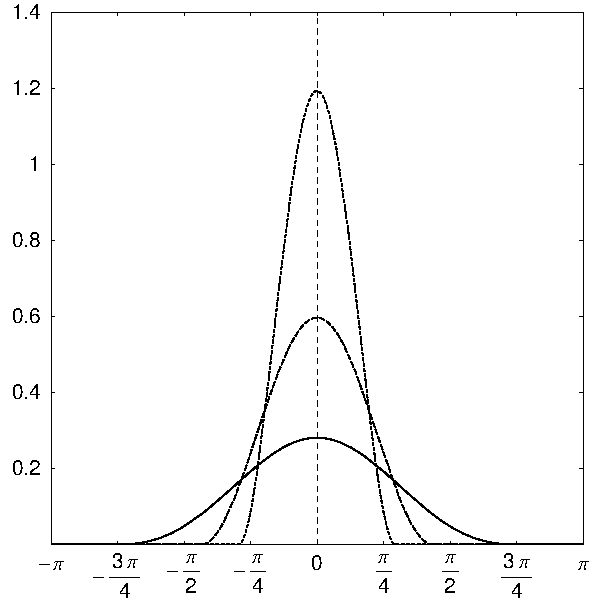
\includegraphics[width=0.45\textwidth]{images/locsup2}}
  \caption{The kernel $L_{h,\lambda}$ for $h = -0.7, 0.2, 0.6$ and different values of $\lambda$.}
  \label{Basics:Figure:LKernel}
\end{figure}

In general, radial functions in $\R^3$ can be restricted to the sphere $\twosphere$. A generic approach
is found in \cite{bahu01} or \cite{cafi}. In the following, we discuss the so-called \emph{spherical Gaussian kernel} 
which takes its name from the bell-shaped Gaussian probability density function.

\begin{definition}
  Let $\sigma \in \Rp$. The \emph{spherical Gaussian kernel}
  $G_{\sigma}:\interv{[}{-1}{1}{]} \rightarrow \R$ is given by
  \begin{equation}
    \label{GaussKernel}
    \nonumber
    \fun{G_{\sigma}}{x} := \e^{\sigma(x-1)}\,.
  \end{equation}
\end{definition}

Figure \ref{Basics:Figure:GKernel} shows the normalized spherical Gaussian kernel
$\fun{\gamma}{\sigma}G_{\sigma}$ with
$\fun{\gamma}{\sigma} := \paren{4\pi}^{-1/2}\paren{\frac{1}{4\sigma}\paren{1-\e^{-4\sigma}}}^{1/2}$ obeying
$\norm{\fun{\gamma}{\sigma}G_{\sigma}}_{\Ln{2}{\twosphere}} = 1$ for different values $\sigma$.

\begin{figure}[tb]
  \centering
   \subfigure[The iterated locally supported kernel $L_{h,\lambda}^{(\mu)}$ for $h = 0.6$, $\lambda = 2$, and $\mu = 1,2,3$.]
   {
     \label{Basics:Figure:LKernelIterated}
     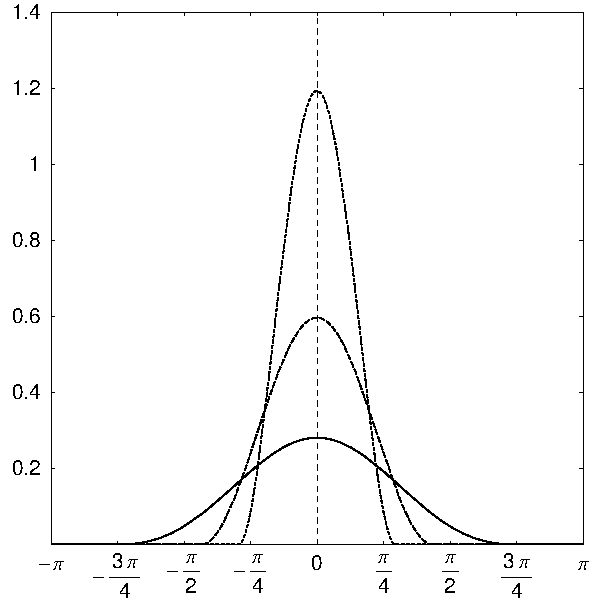
\includegraphics[width=0.45\textwidth]{images/locsup_it}
   }\hfill
   \subfigure[The Gaussian-kernel $\fun{\gamma}{\sigma}G_{\sigma}$ for $\sigma = 2,10,80$.]
   {
     \label{Basics:Figure:GKernel}
     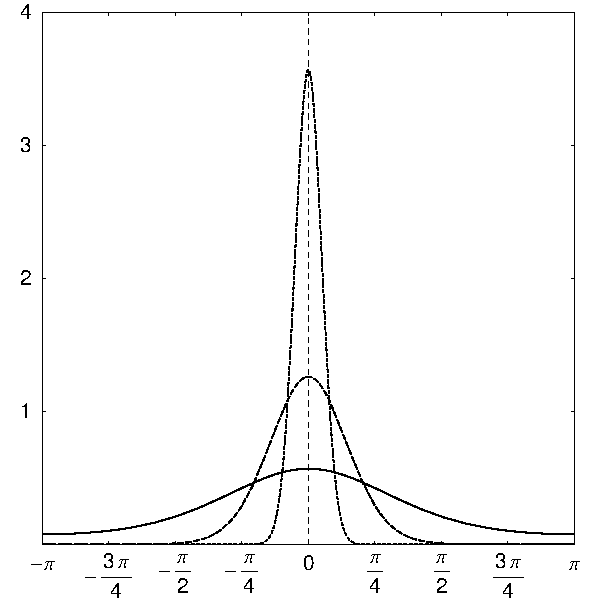
\includegraphics[width=0.45\textwidth]{images/gaussian}
   }
  \caption{}
  \label{Basics:Figure:GLKernel}
\end{figure}

As for the locally supported kernels $L_{h,\lambda}$, the Symbol $\fun{G_{\sigma}^{\wedge}}{k}$ likewise
obeys a three-term recurrence relation. A 'closed' form expression can be given in terms of modified spherical 
Bessel functions of the first kind \cite{bahu01}.
\begin{lemma}${}^{}$\\[-3.5ex]
  \begin{enumerate}
  \item The symbol $\fun{G_{\sigma}^{\wedge}}{k}$ can be computed by a
    recurrence relation
    \begin{equation}
      \label{Basics:Gaussian:SymbolRecurrence}
    \fun{G_{\sigma}^{\wedge}}{k+1} = 
    - \frac{2k+1}{\sigma} \fun{G_{\sigma}^{\wedge}}{k} +
    \fun{G_{\sigma}^{\wedge}}{k-1}   
    \end{equation}
    for $k\in \N$, $\fun{G_{\sigma}^{\wedge}}{0} = 4 \pi \sigma^{-1}
    \e^{-\sigma} \sinh \sigma$, and
    $\fun{G_{\sigma}^{\wedge}}{1} = \frac{2 \pi \paren{\sigma - 1 + 
    \e^{-2\sigma}\paren{1+\sigma}}}{\sigma^2}$.
  \item A 'closed' form of the symbol $\fun{G_{\sigma}^{\wedge}}{k}$ is given by
    \[
      \fun{G_{\sigma}^{\wedge}}{k} = \sigma^{-\frac{1}{2}} \e^{-\sigma}
      \pi^{\frac{3}{2}} \fun{I_{k+\frac{1}{2}}}{\sigma}
    \]
    where $I_{k+\frac{1}{2}}$ denotes the modified Bessel function of the first kind.
    Furthermore, $\fun{G_{\sigma}^{\wedge}}{k} \ge 0$.
  \end{enumerate}
\end{lemma}
\begin{proof}${}^{}$\\[-3.5ex]
  \begin{enumerate}
  \item Integration by parts and the recurrence relation \eqref{three2} yield
    \begin{eqnarray*}
      (2k+1) \fun{G_{\sigma}^{\wedge}}{k} 
      & = & 2\pi \int_{-1}^1 \e^{\sigma{x-1}} (2k+1)\fun{P_{k}}{x} \; \dx x \\
      & = & 2\pi \int_{-1}^1 \e^{\sigma{x-1}} \fun{P_{k+1}'}{x} \; \dx x  - 2\pi \int_{-1}^1 \e^{\sigma{x-1}} \fun{P_{k-1}'}{x} \; \dx x \\
      & = & -\sigma 2\pi \int_{-1}^1 \e^{\sigma{x-1}} \fun{P_{k+1}}{x} \; \dx x  + \sigma 2\pi \int_{-1}^1 \e^{\sigma{x-1}} \fun{P_{k-1}}{x} \; \dx x \\
      & = & -\sigma \fun{G_{\sigma}^{\wedge}}{k+1} + \sigma \fun{G_{\sigma}^{\wedge}}{k-1}.
    \end{eqnarray*}
  \item The solution of the difference equation in \eqref{Basics:Gaussian:SymbolRecurrence} 
  is given by the modified
  Bessel function of the first kind, cf. \cite{bahu01}.
  The nonnegativity follows already from the fact that the spherical Gaussian kernel is a
  positive definite function \cite{powell}.
  \end{enumerate}
  \end{proof}
  
  \begin{remark}
    The forward recurrence relation \eqref{Basics:Gaussian:SymbolRecurrence} proves to be unstable which
    forbids computing the symbol $\fun{G_{\sigma}^{\wedge}}{k}$ in finite precision arithmetic with the 
    desired accuracy. The corresponding backward recurrence relation is stable and in fact, most numerical methods used to
    evaluate Bessel functions rely on backward recursion \cite{prtevefl}. For our 
    numerical tests in Section \ref{Applications:FastSum}, we used Mathematica 5.0 with extended 
    precision arithmetic to compute the coefficients up to double precision accuracy. The GNU 
    scientific library (GSL) also provides subroutines to evaluate various types of Bessel functions \cite{gsldoc}.
    Numerical tests show that their accuracy is sufficient to compete with the coefficients calculated 
    with Mathematica. This provides an easy and reliable means to compute the symbol coefficients
    $\fun{G_{\sigma}}{k}$.
  \end{remark}

\section{Discrete Cosine Transforms}
\label{Basics:DiscreteCosineTransform}

The \emph{discrete cosine transforms (DCTs)} are a class of real transformations closely related to the 
\emph{discrete Fourier transform (DFT)}. They exploit the fact that the 
input data is real and has even symmetry. The Fourier transform of a real-even 
function is real-even and $\mathrm{i}$ times the Fourier transform of a real-odd function is real-odd. 
Similar results hold for the DFT. Based on this fact, one defines 
real transforms respecting the additional symmetry.
Due to the discrete sampling, we have an additional choice: The symmetry can be 
viewed relatively to a data point or to a point halfway between two data points. For our 
purposes, we confine ourselves with introducing two variants.

We define the matrices
\begin{equation}
  \nonumber
  \V{C}_{N} := \paren{\cos \frac{j(2k+1) \pi}{2N}}_{j,k = 0}^{N-1}, \quad \V{D}_N := \diag\, 
  \paren{\varepsilon_j^N}_{j = 0}^{N-1} \quad \paren{N \in \N},
\end{equation}
with $\varepsilon_0^N := \frac{1}{2}$ and $\varepsilon_j^N := 1$ for $j = 1,\ldots,N-1$.
The discrete cosine transforms DCT-II($N$) and DCT-III($N$) are then defined as follows:
\begin{equation}
  \label{Basics:DCT}
  \begin{split}
    \text{DCT-II($N$): } & \R^N \rightarrow \R^N,\ \V{\tilde{a}} := \V{C}_N \: \V{a},\\
    \text{DCT-III($N$): } & \R^N \rightarrow \R^N,\ \V{\tilde{b}} := \V{C}_N^{\transp} \: \V{D}_N \: \V{b}, 
  \end{split}  
\end{equation}
where $\V{a} := \paren{a_k}_{k=0}^{N-1} \in \R^N$ is the input vector and $\V{\tilde{a}} := 
\paren{\tilde{a}_j}_{j=0}^{N-1} \in \R^N$ is the output vector and similarly $\V{b}$ and $\V{\tilde{b}}$. 
The \emph{Chebyshev polynomials of the first kind} $T_{k}$ are given by $\fun{T_{k}}{x} := \fun{\cos}{k \arccos x}$ 
and we obtain
\begin{equation}
  \label{Basics:DCT2}
  \begin{split}
    \tilde{a}_{j} & = \sum_{k = 0}^{N-1} a_{k} \cos \frac{j(2k+1)\pi}{2N} = \sum_{k = 0}^{N-1} a_{k} \fun{T_{j}}{\cos \frac{(2k+1) \pi}{2N}},\\
    \tilde{b}_{j} & = \sum_{k = 0}^{N-1} \varepsilon_k^N b_{k} \cos \frac{k(2j+1)\pi}{2N} = \sum_{k = 0}^{N-1} \varepsilon_k^N b_{k} \fun{T_{k}}{\cos \frac{(2j+1) \pi}{2N}},
  \end{split}  
\end{equation}
for $j = 0,\ldots,N-1$. The following lemma shows that the matrix $\V{C}_N$ is almost orthogonal (for a proof see \cite{bata}).
\begin{lemma}
  \label{Basics:DCT3}
  Let $\V{C}_N$ and $\V{D}_N$ be defined as in \eqref{Basics:DCT}. Then we have
  \[ \V{C}_N \: \V{C}_N^{\transp} \: \V{D}_N = \V{C}_N^{\transp} \: \V{D}_N \: \V{C}_N = \frac{N}{2} \: \V{I}_{N}. \]
\end{lemma}
Therefore the DCT-II is the inverse of the DCT-III and vice versa, up to a scaling factor.

\section{Fast Polynomial Multiplication}
\label{Basics:FastPolynomialMultiplication}
A polynomial $p \in \Pol_{K}$, $K \in \N$ is uniquely determined by its \emph{Chebyshev coefficients} 
$\V{a} := \paren{a_{k}}_{k = 0}^{K}$ with $\fun{p}{x} = \sum_{k=0}^{K} a_{k} \fun{T_{k}}{x}$. Given 
now a second polynomial $q \in \Pol_{K-1}$ with Chebyshev coefficients $\V{b} := \paren{b_{k}}_{k=0}^{K-1}$, 
we give a fast algorithm (see \cite{postta97} and \cite{kupo02}) 
for computing the Chebyshev coefficients $\V{c} := \paren{c_{k}}_{k=0}^{2K-1}$ of the polynomial 
product $r := p \cdot q \in \Pol_{2K-1}$.\\ 
The polynomial $r$ is uniquely determined 
by the products 
\begin{equation}
  \label{Basics:Products}
  f_{j} := \fun{p}{\cos \frac{(2j+1)\pi}{4K}} \fun{q}{\cos \frac{(2j+1)\pi}{4K}}
\end{equation}
for $j = 0,\ldots,2K-1$, and by \eqref{Basics:DCT2} we obtain
\begin{eqnarray*}
  \paren{\fun{p}{\cos \frac{(2j+1)\pi}{4K}}}_{j=0}^{2K-1} = \V{C}_{2K}^{\transp} \: \V{a} = \V{C}_{2K}^{\transp} \:\paren{a_{k}}_{k=0}^{2K-1},\\
  \paren{\fun{q}{\cos \frac{(2j+1)\pi}{4K}}}_{j=0}^{2K-1} = \V{C}_{2K}^{\transp} \: \V{b} = \V{C}_{2K}^{\transp} \:\paren{b_{k}}_{k=0}^{2K-1},
\end{eqnarray*}
where we let $a_{k} := 0$ for $k > K$ and $b_{k} := 0$ for $k > K-1$. This signifies that the evaluation 
of the polynomials $p$ and $q$ can be performed using two DCT-IIIs of lengths $2K$ with an additional 
compensation for the factors $\varepsilon_{k}^K$ introduced by the matrix $\V{D}_{2K}$ in \eqref{Basics:DCT}.
Once calculated the vector of products $\V{f} := \paren{f_{j}}_{j=0}^{2K-1}$ from \eqref{Basics:Products}
and taking into account that by Lemma \ref{Basics:DCT3} one has
$\V{C}_{2K}^{-\transp} = \frac{1}{K} \: \V{D}_{2K} \: \V{C}_{2K}$, we finally find 
\[ 
  \V{c} = \paren{c_{k}}_{k=0}^{2K-1} = \frac{1}{K} \: \V{D}_{2K} \: \V{C}_{2K} \: \V{f}.
\]
This leads to Algorithm \ref{Basics:Algorithm:FastPolynomialMultiplication}. The airthmetic complexity
is $\bigo{K \log K}$ flops owing to the DCT applications.

\begin{algorithm}[tb]
  \caption{Fast Polynomial Multiplication in Chebyshev Representation}
  \label{Basics:Algorithm:FastPolynomialMultiplication}    
  \begin{algorithmic}
    \STATE  Input:  $K \in \N$, Chebyshev coefficients $\paren{a_{k}}_{k = 0}^{K}$,
    $\paren{b_{k}}_{k = 0}^{K-1}$
    \STATE
    \STATE Evaluate the polynomials $p$ and $q$ at the Chebyshev nodes $\paren{\cos \frac{(2j+1)\pi}{4K}}_{j = 0}^{2K-1}$
      using two fast DCT-IIIs of length $2K$.
    \FOR {$j=0,\ldots , 2K-1$} 
      \STATE $f_{j} := \fun{p}{\cos \frac{(2j+1)\pi}{4K}} \fun{q}{\cos \frac{(2j+1)\pi}{4K}}$
    \ENDFOR
    \STATE Compute the Chebyshev coefficients $\paren{c_{k}}_{k=0}^{2K-1}$ of $r$ using a fast DCT-II of length $2K$.
    \STATE
    \STATE Output: Chebyshev coefficients $\paren{c_{k}}_{k=0}^{2K-1}$
    \STATE Complexity: $\bigo{K \log K}$ flops
\end{algorithmic}
\end{algorithm}

\section{Nonuniform Fast Fourier Transform}
\label{Basics:NFFT}

The \emph{nonuniform fast Fourier transform (NFFT)} algorithm generalizes the well known 
\emph{fast Fourier transform (FFT)}. For the sake of simplicity, we restrict 
ourselves here to the one-dimensional case on the torus 
$\mathbb{T} := \R/\Z$ identified with the interval
$[-\pi,\pi)$. For 
fixed $M \in \N_{0}$ and $D \in \N$ we denote by $\mathcal{X} := \pset{\vphi_{j} 
\in [-\pi,\pi)}{|}{j = 0,\ldots,D-1}$ a 
\emph{sampling set} of nodes and let 
$\mathcal{I}^{M} := \pset{k \in \Z}{|}{-\frac{M}{2} 
\le k \le \frac{M}{2}-1}$ be the index set of all `admissible'
\emph{frequencies}. The considered problem is the evaluation of a 
trigonometric polynomial $f: [-\pi,\pi) \rightarrow \C$ with
\begin{equation}
  \label{Basics:NFFT:f}
  \fun{f}{\vphi} := \sum_{k \in \mathcal{I}_{M}} \hat{f}_{k} \e^{\im k x}
\end{equation}
on the sampling set $\mathcal{X}$. The NFFT algorithm is approximative with 
computational complexity $\bigo{M \log M + \fun{\log}{1/\varepsilon}D}$ 
where $\varepsilon$ is the desired accuracy. The technique in use is an 
approximation of the function $f$ in \eqref{Basics:NFFT:f} by a linear 
combination of shifted periodic window functions $\tilde{\varphi}$.
An admissible window function $\tilde{\varphi}$ should be mutually well localized 
in time and frequency.
We refer the interested reader to \cite{st97}, \cite{postta01}, and the references therein.